%%%%%%%%%%%%%%%%%%%%%%%%%%%%%%%%%%%%%%%%%
% Beamer Presentation
% LaTeX Template
% Version 1.0 (10/11/12)
%
% This template has been downloaded from:
% http://www.LaTeXTemplates.com
%
% License:
% CC BY-NC-SA 3.0 (http://creativecommons.org/licenses/by-nc-sa/3.0/)
%
%%%%%%%%%%%%%%%%%%%%%%%%%%%%%%%%%%%%%%%%%

%----------------------------------------------------------------------------------------
%	PACKAGES AND THEMES
%----------------------------------------------------------------------------------------

\documentclass{beamer}
\usepackage{listings}
\usepackage{url}
\usepackage[export]{adjustbox}
\mode<presentation> {
\usepackage{listings}
% The Beamer class comes with a number of default slide themes
% which change the colors and layouts of slides. Below this is a list
% of all the themes, uncomment each in turn to see what they look like.

%\usetheme{default}
%\usetheme{AnnArbor}
%\usetheme{Antibes}
%\usetheme{Bergen}
%\usetheme{Berkeley}
%\usetheme{Berlin}
%\usetheme{Boadilla}
%\usetheme{CambridgeUS}
%\usetheme{Copenhagen}
%\usetheme{Darmstadt}
\usetheme{Dresden}
%\usetheme{Frankfurt}
%\usetheme{Goettingen}
%\usetheme{Hannover}
%\usetheme{Ilmenau}
%\usetheme{JuanLesPins}
%\usetheme{Luebeck}
%\usetheme{Madrid}
%\usetheme{Malmoe}
%\usetheme{Marburg}
%\usetheme{Montpellier}
%\usetheme{PaloAlto}
%\usetheme{Pittsburgh}
%\usetheme{Rochester}
%\usetheme{Singapore}
%\usetheme{Szeged}
%\usetheme{Warsaw}

% As well as themes, the Beamer class has a number of color themes
% for any slide theme. Uncomment each of these in turn to see how it
% changes the colors of your current slide theme.

%\usecolortheme{albatross}
%\usecolortheme{beaver}
%\usecolortheme{beetle}
%\usecolortheme{crane}
%\usecolortheme{dolphin}
%\usecolortheme{dove}
%\usecolortheme{fly}
%\usecolortheme{lily}
%\usecolortheme{orchid}
%\usecolortheme{rose}
%\usecolortheme{seagull}
%\usecolortheme{seahorse}
%\usecolortheme{whale}
%\usecolortheme{wolverine}



\usepackage{wrapfig}

%\setbeamertemplate{footline} % To remove the footer line in all slides uncomment this line
%\setbeamertemplate{footline}[page number] % To replace the footer line in all slides with a simple slide count uncomment this line

%\setbeamertemplate{navigation symbols}{} % To remove the navigation symbols from the bottom of all slides uncomment this line
%
}

\usepackage{graphicx} % Allows including images
\usepackage{booktabs} % Allows the use of \toprule, \midrule and \bottomrule in tables
%----------------------------------------------------------------------------------------
%	TITLE PAGE
%----------------------------------------------------------------------------------------

\title[]{Study and Implementation of a {Decentralized Application} That Can Provide {Permissionless Financial Services} Using an EVM-Based {Blockchain}} % The short title appears at the bottom of every slide, the full title is only on the title page



\author{Mario M. Orozco} % Your name
\institute[HSRM] % Your institution as it will appear on the bottom of every slide, may be shorthand to save space
{
Bachelor Colloquium
\medskip
%\textit{} % Your email address
}

\begin{document}

\begin{frame}
\titlepage % Print the title page as the first slide
\end{frame}


\title[]{Study and Implementation of a \textbf{Decentralized Application} That Can Provide \textbf{Permissionless Financial Services} Using an EVM-Based \textbf{Blockchain}}

\begin{frame}
	\titlepage % Print the title page as the first slide
\end{frame}


\begin{frame}
\frametitle{Contents} % Table of contents slide, comment this block out to remove it
\tableofcontents % Throughout your presentation, if you choose to use \section{} and \subsection{} commands, these will automatically be printed on this slide as an overview of your presentation
\end{frame}

%----------------------------------------------------------------------------------------
%	PRESENTATION SLIDES
%----------------------------------------------------------------------------------------
%------------------------------------------------
\section{Goals}
\begin{frame}
\frametitle{Goals}
The \textbf{goals} of the Thesis were to provide a better understanding of:
\linebreak
\begin{itemize}
	\item[$\bullet$] The way that decentralized applications or \textbf{dapps} are \textbf{built}. \\ 
	\item[$\bullet$] The used \textbf{technology}.\\ 
	\item[$\bullet$] \textbf{Developing} \textbf{a} \textbf{Dapp} that uses well-known DeFi protocols, to let users access
	permissionless financial services such as lending and borrowing of crypto
	assets.\\ 
\end{itemize}
\end{frame}

%------------------------------------------------
\section{Blockchain}
\begin{frame}
\frametitle{Blockchain}
\includegraphics[width=0.3\textwidth,center]{bc}
\linebreak
\linebreak
%The term blockchain usually refers to a set of nodes, of a \textbf{peer-to-peer %network}, running the \textbf{consensus protocol}. Where every node holds a copy of the %blockchain. 
The term blockchain usually refers to a \textbf{public ledger} of transaction records, \textbf{shared and synchronized} by \\a\textbf{ peer-to-peer network}, and a \textbf{consensus protocol}.
\end{frame}


\begin{frame}
\frametitle{But what is a blockchain?}
\includegraphics[width=0.1\textwidth,right]{bc}
\includegraphics[width=0.79\textwidth,center]{../images/bc}
\begin{itemize}
	\item[$\bullet$] Is a type of \textbf{database} (\textbf{append-only, read only} data structure), that stores
	data in 'blocks'.
	\item[$\bullet$] Blocks are chronologically ordered by discrete timestamps and
	linked to each other using \textbf{Cryptographic Hash Functions}.
	\item[$\bullet$] \textbf{CHF} and \textbf{Merkle Trees} ensure the integrity of the blockchain.
\end{itemize}
\end{frame}

\begin{frame}
	\frametitle{Cryptographic Hash Functions (CHF)}
	A cryptographic hash function maps a given data of \textbf{variable size to a fixed length} \emph{n}-bit string \textit{(hash value)}. $ H : \{0,1\}^* \to \{0,1\}^n $.
	\linebreak
	\linebreak
	\includegraphics[width=0.99\textwidth,center]{chf}					
\end{frame}

\begin{frame}
	\frametitle{CHF Properties}
	\begin{itemize}
		\item[$\bullet$] \textbf{Collision resistance:} Computationally infeasible $ O(2^\frac{n}{2})$ that different inputs, i.e., blocks of data, will generate the same hash value.\linebreak
		\item[$\bullet$] \textbf{Preimage resistance:} Computationally infeasible $ O(2^n)$ to retrieve the input data from its hash value (one-way function).\linebreak
		\item[$\bullet$] \textbf{Second preimage resistance:} For a given hash value, it is computationally infeasible $ O(2^n) $ to find another input, i.e., a block data input, that generates the same hash value.
	\end{itemize}		
\end{frame}


\begin{frame}
	\frametitle{Merkle Tree}
	\includegraphics[width=0.6\textwidth, center]{../images/merkle}

\begin{itemize}
	\item[$\bullet$] Binary Tree: Efficient Data Structure: $2log (N)$.

	\item[$\bullet$] Constructed bottom-up.
\end{itemize}
\end{frame}




\begin{frame}
	\frametitle{Consensus Protocol}
	\includegraphics[width=0.15\textwidth,right]{bc}
	The most common consensus mechanisms are:\linebreak
	\begin{itemize}
		\item[$\bullet$] \textbf{Proof of work (PoW)}: Nodes have to solve a cryptographic task in order to
		validate a block; the first node to find a solution can submit the transaction.
		\linebreak
		\item[$\bullet$] \textbf{Proof of stake (PoS)}: The node that can validate a transaction is randomly
		selected, depending on the "stake" that a node has on the network.
	\end{itemize}	
	
\end{frame}

\begin{frame}
\frametitle{Bitcoin Example}

\noindent\begin{minipage}{0.6\textwidth}% adapt widths of minipages to your needs
	\includegraphics[width=\linewidth]{btcblocks}
\end{minipage}%
%\hfill%
\begin{minipage}{0.3\textwidth}\raggedleft
	SHA-256,\\
	POW
\end{minipage}

	%\includegraphics[width=0.6\textwidth, center]{btcblocks}
\end{frame}

\begin{frame}
	\frametitle{Bitcoin}
	%\includegraphics[width=0.1\textwidth, right]{bc}
The distributed computation system that bitcoin\\ introduced: a \textbf{proof-of-work} algorithm to produce a consensus in a distributed system without a central trusted authority, in combination with the blockchain storage system, solved the \textbf{double-spend problem} and the \textbf{Byzantine generals problem}.
\linebreak
\linebreak	
\linebreak
\linebreak
\end{frame}

%------------------------------------------------
\section{Ethereum}
\begin{frame}
\frametitle{Ethereum}
\includegraphics[width=0.1\textwidth,right]{bc}
Ethereum is a decentralized computing platform or a \textbf{decentralized pseudo-turing complete virtual machine}, \\which runs \textbf{smart contracts} and stores its state changes in its blockchain.
\end{frame}

\begin{frame}
	\frametitle{Ethereum Virtual Machine (EVM)}
	\includegraphics[width=0.65\textwidth, center]{../images/evm}
	\begin{itemize}
		\item[$\bullet$] A quasi-Turing-complete machine.
		\item[$\bullet$] The quasi means that its computation is limited by the available \textbf{gas} that the executed contract has.
	\end{itemize}
\end{frame}



\begin{frame}
	\frametitle{Ether and Gas}
	\begin{itemize}
		\item[$\bullet$] Ether (ETH) is the native cryptocurrency of Ethereum.
		\item[$\bullet$] ETH is used to pay for transaction fees or EVM computing power in the form of gas units.
		\item[$\bullet$] The gas unit is represented in \textit{gwei}, and is set by the participants of the consensus protocol (miners), based on the supply and demand of the network computational power.
		\item[$\bullet$] For instance, with an average gas price of 15 gwei, and $G_{transaction} = 21000$, sending a transaction would cost: $21000*15 = 315000~Gwei$ or $0.000315~Ether.$
	\end{itemize}

\begin{table}[htp]
	\centering
	%\begin{center}
	\begin{tabular}{|l|l|l|}
		\hline
		\multicolumn{1}{|c|}{\textbf{Unit Name}} & 
		\multicolumn{1}{|c|}{\textbf{Wei Value}} \\\hline
		$Ether$ & $1^{18}$  \\\hline
		$Gwei$  & $1^{9}$  \\\hline
		$Wei$   & $1$     \\\hline   
	\end{tabular}
	%\end{center}
\end{table}

\end{frame}


\begin{frame}
	\frametitle{Smart Contracts}
	\begin{itemize}
		\item[$\bullet$] A \textbf{computer program} executed by the EVM.
		\item[$\bullet$] Smart Contracts \textbf{have a balance and can send transactions} in the form of messages.
		\item[$\bullet$] Characteristics: \textbf{Immutability}, \textbf{Determinism}, \textbf{Limitations}, \textbf{Lifecycle}, \textbf{Composability}, \textbf{Permissionless}.
	\end{itemize}
\end{frame}


\begin{frame}
	\frametitle{Tokens}
	\begin{itemize}
		\item[$\bullet$]  In the context of Ethereum, a token is a \textbf{digital representation} or abstraction of something that lives on the Blockchain.
		\item[$\bullet$] For instance, tokens can represent \textbf{currencies}, \textbf{shares in a company}, or even a \textbf{virtual pet}. 
		\item[$\bullet$] Unlike Ether, which is managed by the Ethereum protocol, tokens are \textbf{created and handled by smart contracts}. 
		\item[$\bullet$] Everyone can create a token. However, some \textbf{standards} need to be followed \textbf{for the creation of tokens}. 
		\item[$\bullet$] \textbf{ERC20} Token Standard, for the representation of \textbf{fungible tokens}. For instance, a token that represents a currency or a share in a company. 
	\end{itemize}
\end{frame}



\begin{frame}
\frametitle{Decentralized Applications (Dapps)}
\noindent\begin{minipage}{0.45\textwidth}% adapt widths of minipages to your needs
	\includegraphics[width=\linewidth]{../images/dappcomponents1}
\end{minipage}%
%\hfill%
\begin{minipage}{0.55\textwidth}\raggedleft
	\begin{itemize}
	\item[$\bullet$] A dapp has its backend running on a decentralized peer-to-peer network like Ethereum.
	\linebreak
	\linebreak
	\item[$\bullet$] The backend is smart contracts executed by the EVM\rightarrow same properties as smart contracts.
\end{itemize}

\end{minipage}	
	
	

	%\includegraphics[width=0.4\textwidth, center]{../images/dapp}

\end{frame}



%------------------------------------------------
\section{Decentralized Finance (DeFi)}

\begin{frame}	
\frametitle{Decentralized Finance (DeFi) }
	\begin{itemize}

		\item[$\bullet$] Decentralized finance or DeFi refers to a set of \textbf{dapps} that are \textbf{focused on financial services}. 
		\item[$\bullet$] The term finance involves the creation, and management of money, in \textbf{traditional finance systems} this is done by financial institutions(Banks), which emit, buy and sell financial instruments(cash, bonds, loans...) on financial markets(exchanges), all \textbf{regulated by Laws}. 
		\item[$\bullet$] In \textbf{DeFi}, these practices and processes are determined by protocols that \textbf{rely on smart contracts}, which means Defi is an open, permissionless, and composable stack of protocols built on top of a blockchain such as Ethereum.
	\end{itemize}
\end{frame}

\begin{frame}	
	\frametitle{Decentralized Finance (DeFi) }
	\begin{itemize}
		\item[$\bullet$]  DeFi has gained a lot of traction in the past years
		and according to Defipulse, the Total Locked Value or TVL (held by smart contracts) in all the DeFi applications and protocols today is: $~40$B USD \\
		\includegraphics[width=0.95\textwidth, center]{tvl}
	\end{itemize}
\end{frame}

\begin{frame}	
	\frametitle{Maker Protocol}
	\begin{itemize}
		\item[$\bullet$] One \textbf{essential piece of DeFi is stablecoins}.
		\item[$\bullet$] \textbf{Stablecoins} are cryptocurrencies \textbf{pegged} to a \textbf{predetermined} \textbf{value}, usually to the USD value. 
		\item[$\bullet$] Stablecoins enable DeFi users to access more traditional assets, \textbf{avoid}ing the natural \textbf{volatility of crypto assets}.
		\item[$\bullet$] The \textbf{Maker Protocol} is a project built on Ethereum that \textbf{allows users to generate the stablecoin DAI}.
		\item[$\bullet$] DAI is \textbf{pegged to the USD} value and collateral backed by different crypto assets authorized by the MakerDao, for instance, ETH.
		\item[$\bullet$] Example: The Maker ETH-C Vault has a minimum collateral ratio of 170\%, meaning that for every \$170 of ETH deposit in the Vault a maximum of 100 DAI can be generated.
	\end{itemize}
\end{frame}

\begin{frame}	
	\frametitle{Aave Protocol}
	\begin{itemize}
		\item[$\bullet$] Aave is a DeFi liquidity protocol that \textbf{enables users to lend and borrow}
		crypto assets.
		\item[$\bullet$]  Users that supply liquidity to the protocol (\textbf{lenders}) \textbf{earn interest} on their deposited assets, and \textbf{borrowers} are able to \textbf{borrow crypto assets after depositing collateral} to the pool contract. 
		\item[$\bullet$]  The \textbf{interest rate} for users (borrowers and lenders) is decided \textbf{algorithmically based on the reserves} available in the pool.
	\end{itemize}
\end{frame}

\begin{frame}	
	\frametitle{Aave Protocol}
	\includegraphics[width=0.7\textwidth, center]{../images/lp_reserves}
	\begin{itemize}
		\item[$\bullet$] The \textbf{reserves} are the multiple currencies deposited on the pool expressed in ETH value.
	\end{itemize}
\end{frame}

\begin{frame}	
	\frametitle{Aave Protocol: Rates and Risk Parameters}
	%\includegraphics[width=0.65\textwidth, center]{../images/lp_reserves}
	\begin{itemize}
		\item[$\bullet$] The \textbf{interest rate}, for lenders and borrowers, is \textbf{determined by} the \textbf{status} of the specific \textbf{reserve}.
		\item[$\bullet$] For \textbf{lenders}, the interest rate depends on  the \textit{current liquidity rate}: $ R_{t} = R_{o}U $, where $ R_{o} $ is the overall \textbf{borrow rate} of the reserve.
	\end{itemize}
\begin{equation}
	R_{o} = 
	\left\{\begin{matrix}
		&  0~~if~~B_{t}=0\\ 
		& \frac{B_{v}R_{v}+ B_{s}R_{sa}}{B_{t}}~~if~~B_{t} > 0
	\end{matrix}\right.
\end{equation}
\end{frame}

\begin{frame}	
	\frametitle{Aave Protocol: Rates and Risk Parameters}
	%\includegraphics[width=0.65\textwidth, center]{../images/lp_reserves}
	\begin{itemize}
		\item[] With the \textbf{total} amount of \textbf{borrowed} liquidity $B_{t} $ (\textit{total borrows}), expressed as the sum of the \textbf{total stable borrows} \textbf{plus}  the \textbf{total variable borrows} :
		\[ B_{t} = B_{s}+B_{v} \]
		And $ U $ is the \textit{utilization rate}, which is the representation of the \textbf{utilization of the deposited assets}, defined as follows:
		\begin{equation}
			U = 
			\left\{\begin{matrix}
				&  0~~if~~L_{t}=0\\ 
				& \frac{B_{t}}{L_{t}}~~if~~L_{t} > 0
			\end{matrix}\right.
		\end{equation}
		Where $L_{t}$  is the \textit{total liquidity} available in the reserve.
	\end{itemize}

\end{frame}

\begin{frame}	
	\frametitle{Aave Protocol: Rates and Risk Parameters}
	%\includegraphics[width=0.65\textwidth, center]{../images/lp_reserves}
	\begin{itemize}
		\item[] \textbf{Loan-To-Value (LTV)}
		\linebreak
		\item[$\bullet$] A user will be able to borrow a maximum amount depending on the Loan-To-Value of the desired asset reserve. 
		\item[$\bullet$] For instance, if the LTV value of a given asset is  60\%, for every 1 ETH value of collateral, a user can borrow a maximum of 0.6 ETH value of the desired asset reserve.
	\end{itemize}
	
\end{frame}

\begin{frame}	
	\frametitle{Aave Protocol: Rates and Risk Parameters}
	%\includegraphics[width=0.65\textwidth, center]{../images/lp_reserves}
	\begin{itemize}
		\item[] \textbf{Liquidation Threshold}
		\linebreak
		\item[$\bullet$] The percentage at which a borrow position can be liquidated.
		\item[$\bullet$] For instance, if the liquidation threshold of a given asset is 80\% and the borrow position value surpasses 80\% of the collateral value, the position can be liquidated.
	\end{itemize}
	
\end{frame}


\begin{frame}	
	\frametitle{Aave Protocol: Rates and Risk Parameters}
	%\includegraphics[width=0.65\textwidth, center]{../images/lp_reserves}
	\begin{itemize}
		\item[] \textbf{Liquidations}
		\linebreak
		\item[$\bullet$] To maintain the solvency of the protocol, anyone can liquidate a borrow position, i.e., buy a maximum of 50\% of the borrow position.
		\item[$\bullet$] Every liquidated position has a liquidation bonus, which depends on the asset. 
		\item[$\bullet$] For instance, if someone borrows 1 ETH worth of DAI and its~$H_{f}$~\ drops below 1, anyone can liquidate the position (max 50\%) for a bonus of 5\% (105\% liquidation ratio), and the liquidator can claim up to 0.5 + 0.05 ETH by repaying 0.5 ETH worth of DAI.
	\end{itemize}
	
\end{frame}

\begin{frame}	
	\frametitle{Aave Protocol: Rates and Risk Parameters}
	%\includegraphics[width=0.65\textwidth, center]{../images/lp_reserves}
	\begin{itemize}
		\item[] \textbf{Health Factor}
		\linebreak
		\item[$\bullet$] Indicates if the borrow position of the user can be liquidated.
		If~$H_{f} < 1$, the borrow position can be liquidated.
		\[ H_{f} = \frac{\sum Collateral_{i}~in~ETH~\times Liquidation Threshold_{i}}{Total~Borrows~in~ETH} \]
		
	\end{itemize}
	
\end{frame}


%------------------------------------------------
\section{Implementation}

\begin{frame}
\frametitle{Implementation}
\includegraphics[width=0.6\textwidth, center]{../images/USECASE-full_nofl1}
\end{frame}

\begin{frame}
	\frametitle{Interaction with the Smart Contracts}
	\includegraphics[width=0.8\textwidth, center]{../images/interactionSC}
\end{frame}

\begin{frame}
	\frametitle{Interaction with the users}
	\includegraphics[width=0.75\textwidth, center]{../images/thesis-dapp1}
\end{frame}

\begin{frame}
	\frametitle{Implementation: Example deposit DAI}
	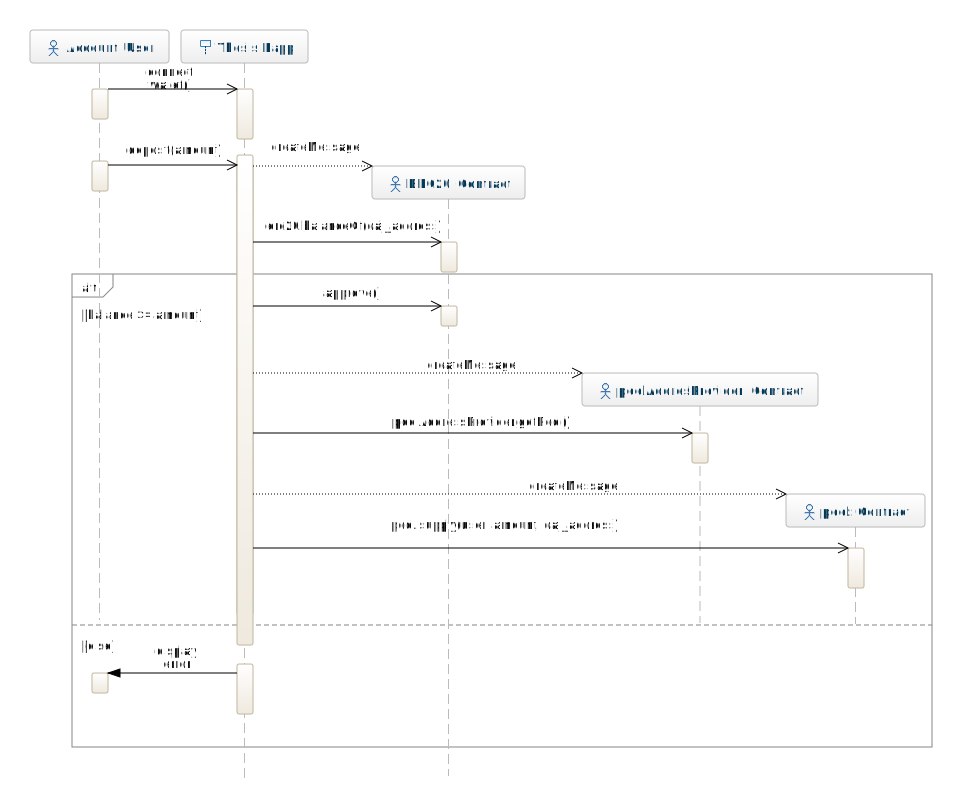
\includegraphics[width=0.8\textwidth, center]{../images/sequence-deposit}
\end{frame}

%------------------------------------------------
\section{Demo}

\begin{frame}
\frametitle{Live Demo}
\includegraphics[width=0.8\textwidth, center]{demo}
\end{frame}

%------------------------------------------------

\section{Conclusions}

\begin{frame}
\frametitle{Conclusions}
\begin{itemize}
	\item[$\bullet$]  \textbf{Achieved Goals}
	\item[$\bullet$]  \textbf{Challenges}
	\item[$\bullet$]  \textbf{Future work}
	\item[$\bullet$]  \textbf{Personally}
\end{itemize}
\end{frame}


\section{Questions}

\begin{frame}
\frametitle{Questions}

\Huge{\centerline{Thanks!}}
\end{frame}

%-------- EXTRAS


\section{}

\begin{frame}
	\frametitle{Extras}
	
\end{frame}

\begin{frame}
	\frametitle{Ethereum has an account-based model}
	\begin{itemize}
		\item[$\bullet$] Every \textbf{account} represents a \textbf{state}.
		\item[$\bullet$] An account is \textbf{mapped with} a 160 bits address (\textbf{public key}).
		\item[$\bullet$] \textbf{Two types} of accounts: Externally owned account (\textbf{EOA}), controlled by a private key and (smart) \textbf{contract account}, controlled by EVM code.
	\end{itemize}
\end{frame}

\begin{frame}
	\frametitle{Ethereum has an account-based model}
	\includegraphics[width=0.8\textwidth, center]{../images/accounts}
	
\end{frame}

\begin{frame}
	\frametitle{Transactions and Messages}
	\begin{itemize}
		\item[$\bullet$] Two types of transactions: \textbf{Message calls}, \textbf{Contract creations}. \linebreak
		\item[$\bullet$] \textbf{Messages} can be seen as \textbf{internal transactions between contracts} triggered by a message call.
	\end{itemize}
\end{frame}




\begin{frame}
	\frametitle{Consensus Protocol}
	\includegraphics[width=0.15\textwidth,right]{bc}
	Who can append a new data block?\linebreak
	\begin{itemize}
		\item[$\bullet$] \textbf{Any participant} or node of the network, depending on the blockchain type, \textbf{can append a new block}.\linebreak
		\item[$\bullet$] \textbf{Participants} on the blockchain \textbf{must verify} any transaction according to the set of rules or consensus protocol of the blockchain network.
	\end{itemize}				
\end{frame}
\begin{frame}
	\frametitle{Tokens}
	\begin{itemize}
		\item[$\bullet$] \textbf{ERC20} Token Standard, for the representation of \textbf{fungible tokens}. For instance, a token that represents a currency or a share in a company. 
		\linebreak
		\linebreak
		\item[$\bullet$] The \textbf{ERC721} Token Standard, for \textbf{non-fungible tokens} or representation of unique goods like an ID or collectibles.  
	\end{itemize}
\end{frame}

\begin{frame}
	\frametitle{Solidity}
	\begin{itemize}
		\item[$\bullet$]  Solidity is an object-oriented or contract-oriented high-level programming Language, designed to \textbf{target the EVM}.
		\item[$\bullet$] The \textbf{Solidity compiler} converts Solidity contracts into \textbf{EVM bytecode} and generates the contract \textbf{Application Binary Interface (ABI)}, which enables the interaction with contracts.
	\end{itemize}
\end{frame}


\begin{frame}	
	\frametitle{Aave Protocol: Tokenization, aTokens}
	%\includegraphics[width=0.65\textwidth, center]{../images/USECASE-full_nofl1}
	\begin{itemize}
		\item[$\bullet$] Aave Tokens or \textbf{aTokens} are ERC20 tokens that lenders, and borrowers, receive once the deposit or borrow transaction is processed. 
		\item[$\bullet$] aTokens \textbf{maps 1:1}, the deposited or borrowed asset, also known as the underlying asset. 
		\item[$\bullet$] For instance, if a user deposits 100 DAI, 100 aDAI is sent to its account.
		\item[$\bullet$] The balance of a specific aTokens changes depending on the interest rate of the underlying asset.
		
	\end{itemize}
	
\end{frame}
%----------------------------------------------------------------------------------------

\end{document} 